\documentclass[11pt,a4paper]{article} %% 1.Ebene = chapter, headings

\usepackage[utf8]{inputenc} 
\usepackage[T1]{fontenc} 
\usepackage{lmodern}
\usepackage{tcolorbox}

\usepackage[german]{babel}


\setlength{\parindent}{0pt}
\setlength{\parskip}{1ex plus 0.5ex minus 0.5ex}

\usepackage{amsmath} 


\usepackage{graphicx} 

\usepackage[section]{placeins}
\usepackage{booktabs}


\usepackage{hyperref}
\hypersetup{
	colorlinks,
	citecolor=red,
	filecolor=black,
	linkcolor=black,
	urlcolor=black}
\graphicspath{}

\begin{document}



{
	\centering 
	\large 
	Physiklabor für Anfänger*innen \\
	Ferienpraktikum im Sommersemester 2018 \\[4mm]
	\textbf{\LARGE 
		Versuch 22: Kreiselpräzession
	} \\[3mm]
	(durchgeführt am 21.09.2018 bei Adrian Hauber) \\
	Ye Joon Kim, Marouan Zouari\\
	\today \\[10mm]
}

\section{Einführung}
Ein schräger Kreisel, auf den eine Gravitationskraft wirkt, führt eine Präzession aus, da das auf den Kreisel wirkenden Drehmoment verursacht eine Änderung des Drehmoments senkrecht zur Kraft und Figurenachse.

Das Drehmoment ist definiert als die Zeitliche Änderung des Drehimpulses. 
\begin{equation}
\vec{M} = \frac{d\vec{L}}{dt}
\end{equation}
und das Drehimpuls lässt auch sich in diesem Fall schreiben als:
\begin{equation}
\vec{M} =\vec{r}\times\vec{G}
\end{equation}

Mit Geometrie kann $dL$ in Terme von $d\varphi$ geschrieben werden (Siehe Abbildung). Da die Präzissionsgeschwindigkeit $\frac{d\varphi}{dt}$ ist, kann $\omega_P$ geschrieben werden als:
$$\omega_P = \frac{dL}{dt\cdot L\cdot \sin\theta}$$
und deshalb:
$$\frac{d\vec{L}}{dt} = \vec{\omega_P}\times \vec{L}$$
und mit Gleichung (1) und (2):
$$\vec{r}\times \vec{G} = \vec{\omega_P}\times \vec{L}$$
Angenommen, dass die Rotationsgeschwindigkeit, $\omega_F$, viel größer ist als die Präzessionsgeschwindigkeit, $\omega_P$ ist, können $\vec{L}$ zu $I_A\vec{\omega}_A$ und $\omega_A$ zu $\omega_F$ angenähert werden. Wobei $\vec{L}$ die Drehmoment, $I_A$ die Trägheitsmoment entlang der Figurenachse und $\omega_A$ der Anteil der Gesamt-Winkelgeschwindigkeit entlang der Figurenachse sind. Wenn man nur die Beträge betrachtet, kann die obige Formel zu 
\begin{equation}
I_A = \frac{rG}{\omega_F \omega_P}
\end{equation}
umgeformt werden.

\section{Ziel des Versuchs}
Das Ziel dieses Versuchs ist es, das Trägheitsmoment des Kreisels entlang der Figurenachse durch die Messung der Präzessions- und Rotationsgeschwindigkeiten zu bestimmen.

\section{Aufbau}

\begin{figure}[h]
	\centering
	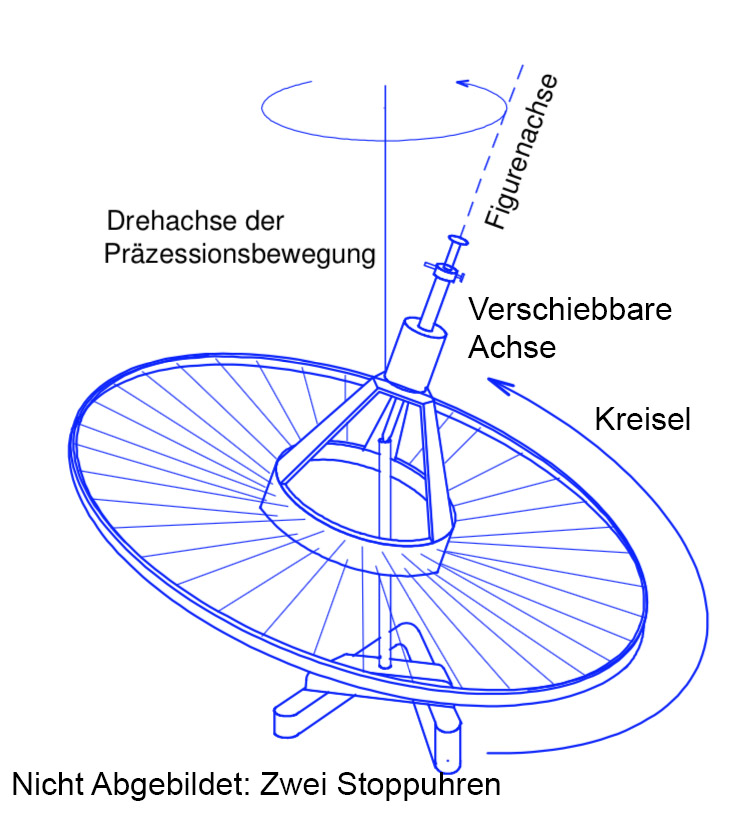
\includegraphics[scale=0.5]{Abb}
	\caption{Aufbau zum Versuch ("Versuchsanleitungen")}
\end{figure}
\section{Durchführung}

\section{Auswertung und Fehleranalyse}
Zur Bestimmung des Trägheitsmoments entlang der Figurenachse wird die oben hergeleitete Formel benutzt, nämlich:
$$I_A = \frac{rG}{\omega_F \omega_P}$$

Zuerst wurden die Werte für $\omega_F$ und $\omega_P$ für die verschiedene $x$ und Messreihen bestimmt (Siehe Anhang 1). 
\begin{tcolorbox}[colback=white]
\subsubsection{Rechenweg}
Für die Bestimmung von $\omega$ wurde die folgende Formel benutzt:
$$ \omega = \frac{T_\textrm{Tot}}{n}\frac{1}{2\pi}$$
Wobei $T_\textrm{Tot}$ die gesamte Zeitdauer der Messung, und $n$ die Anzahl Drehungen war.
Für den Fehler wurde der Messfehler durch $sqrt{n}$ geteilt, da es handelt sich um einen Mittelwert.
\end{tcolorbox}

Um den Offset zwischen $x$, der Skala auf der Kreiselachse, und $r$, der Abstand zwischen den Schwerpunkt und Unterstützungspunkt zu bestimmen wurde $\frac{\omega_F\omega_P}{G}$ gegen $x$ aufgetragen. Der x-Achsenabschnitt is dann der Offset zwischen $x$ und $r$, da nach Gleichung (3) sollen $\frac{\omega_F\omega_P}{G}$ proportional zu $r$ sein und die Fit-Kurve den Nullpunkt schneiden. Die Steigung entspricht dann $-\frac{1}{I_A}$. Da Gleichung (3) lässt sich umformen als:
$$ \frac{\omega_F\omega_P}{G}  = \frac{1}{I_A} r$$. Es ist hier zu beachten, dass die Steigung negativ ist, da die Werte für $x$ und $r$ in andere Richtungen gemessen werden. Die Berechnung wurde mit einem Excel-Dokument und die Darstellung mit Logger-Pro gemacht (Siehe Abbildung 2).


\begin{tcolorbox}[colback=white] 
\subsubsection{Rechenweg}
Zuerst wurden die Werte für $\frac{\omega_F\omega_P}{G}$ für alle Messreihen berechnet. Die Fehler für $\frac{\omega_F\omega_P}{G}$ wurden mit der Formel für die Standardabweichung bestimmt, nämlich:
$$s_x = \sqrt{\frac{\sum_{i=1}^{n}(x_i-\bar{x})^2}{n-1}} $$
\end{tcolorbox}

\begin{figure}
	\centering
	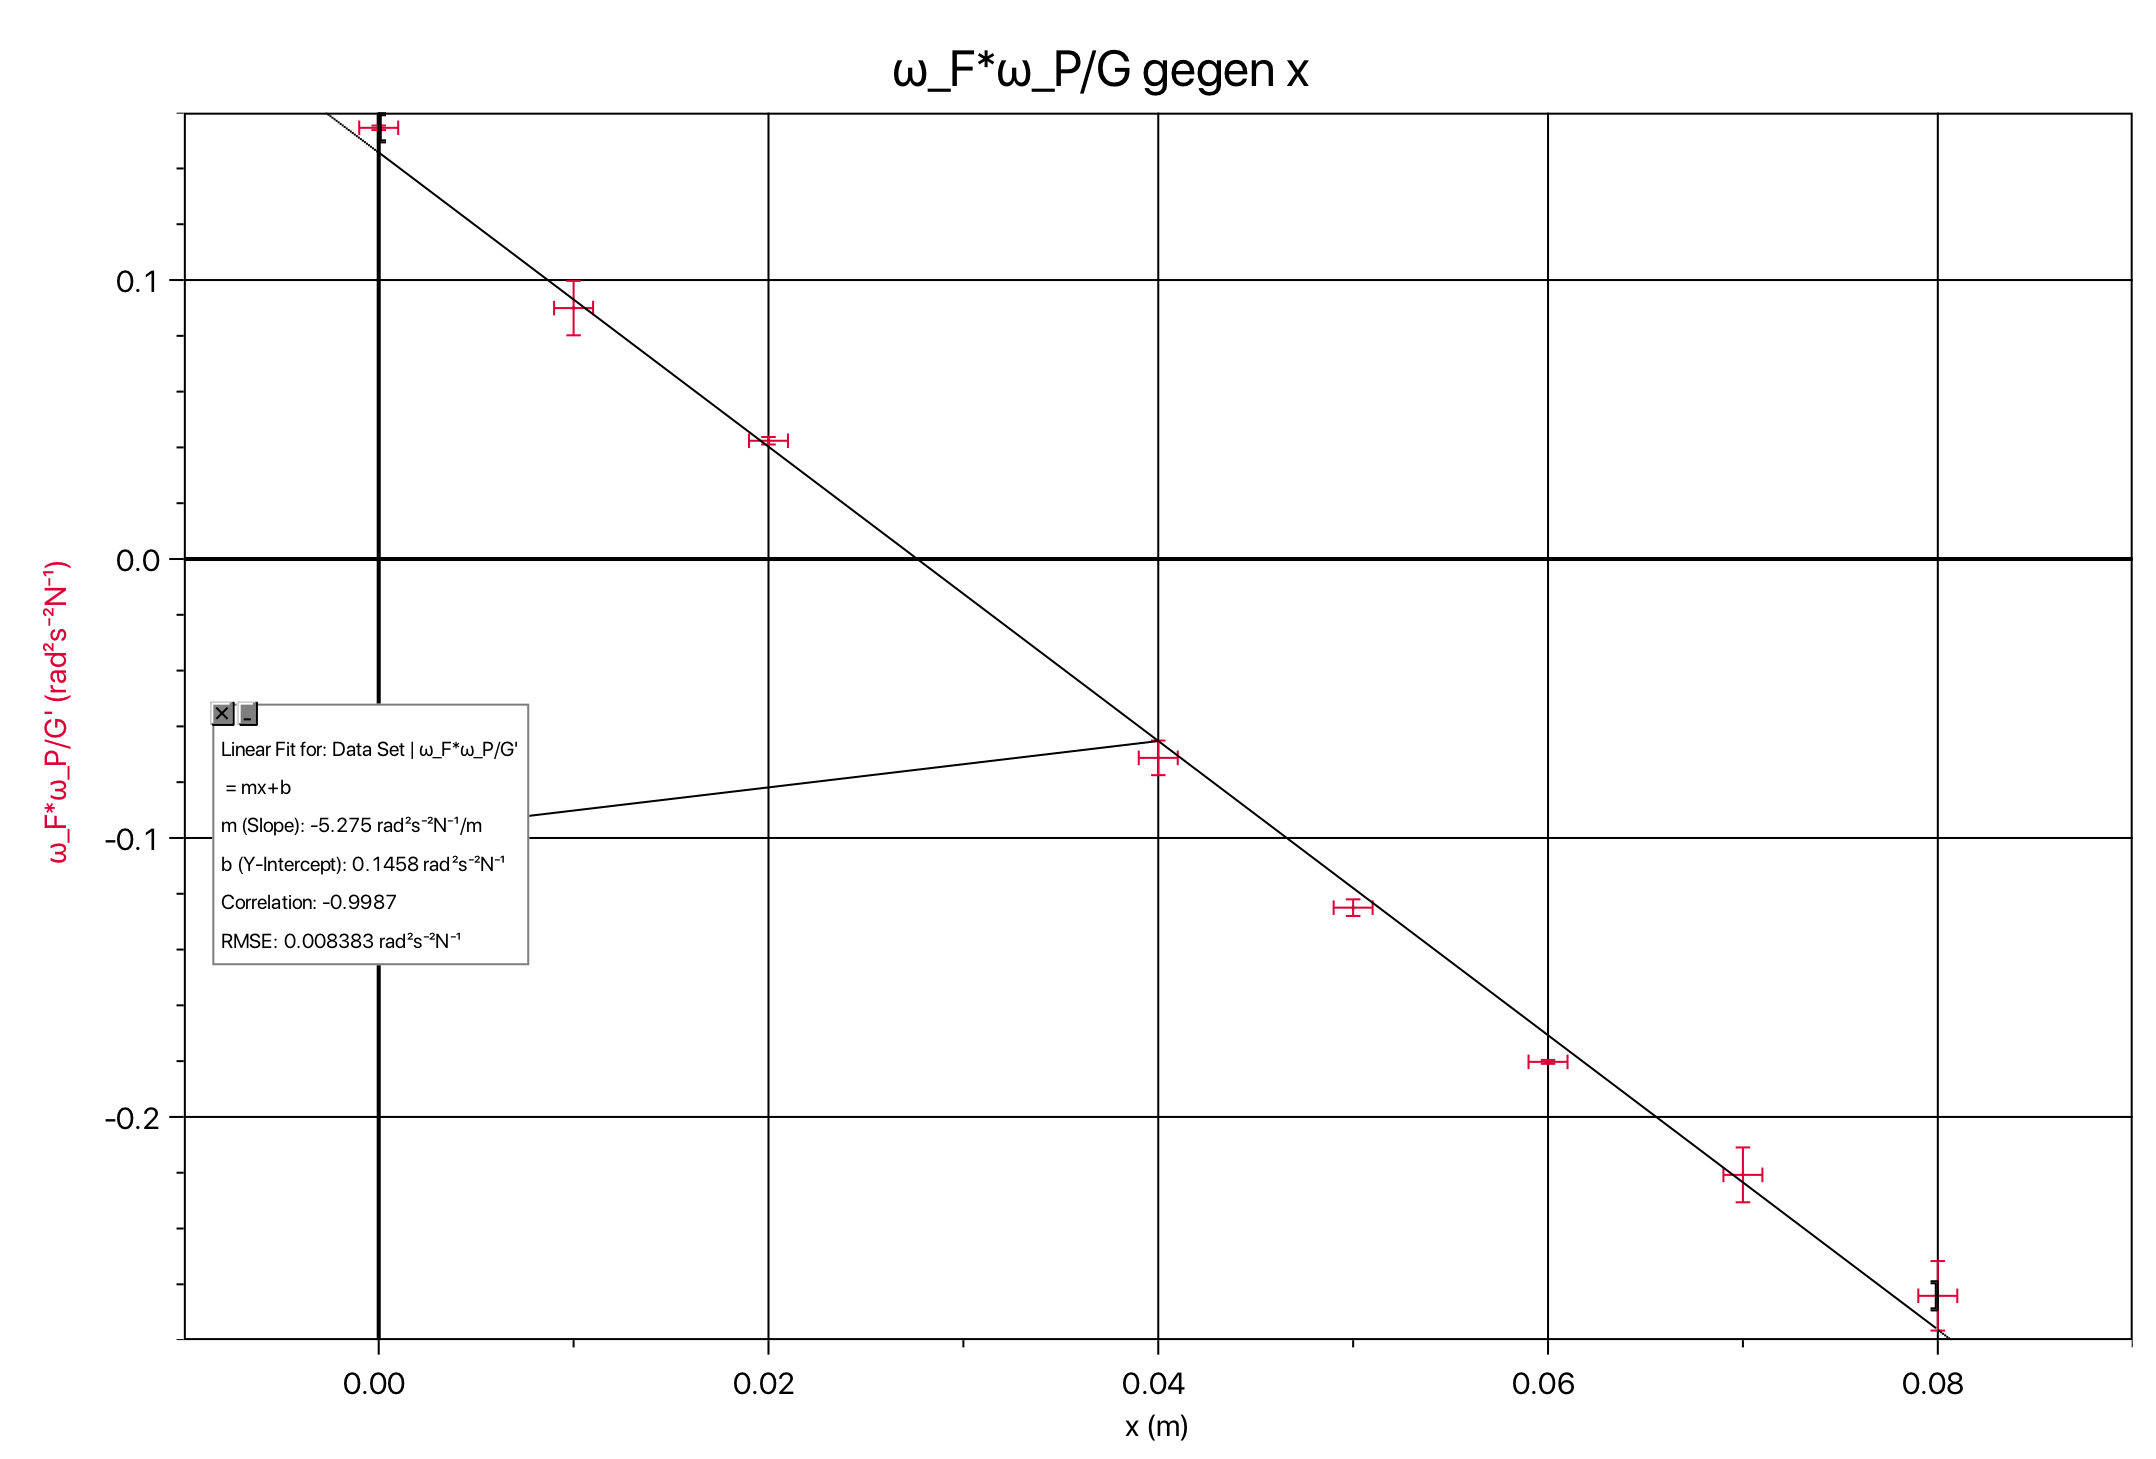
\includegraphics[width=\linewidth]{Abb1}
	\caption{Eine Graph von $\frac{\omega_F\omega_P}{G}$ als Funktion von $x$}
\end{figure}
Das Trägheitsmoment entlang der Figurenachse ist deshalb:
$$I_A = (0,190 \pm 0,004) \textrm{kgm}^2$$

Die Unsicherheit wurde mit der Vereinfachten Formel für Produkte und Quotienten berechnet. 
\section{Diskussion der Ergebnisse}
Der berechnete Wert für $I_A$ ist:
$$I_A = (0,190 \pm 0,004) \textrm{kgm}^2$$

Da es keinen Literatur- oder direkt gemessenen Wert für das Trägheitsmoment des Kreisels gibt, kann keinen direkten Vergleich gemacht werden. Trotzdem kann ein Maximalwert berechnet werden, indem man den Idealfall betrachtet. Für einen idealen Hohlzylinder, ist sein Trägheitsmoment $I = mr^2$. Deswegen ist das maximale theoretische Trägheitsmoment des Kreisels 0,32 kgm$^2$, angenommen, dass der Durchmesser des Kreisels nicht größer als 0,5 Meter war. In der Realität ist das Trägheitsmoment viel kleiner als dieser Wert, da ein Kreisel hat auch Masse innerhalb des Radius. Da der gemessene Wert kleiner als dieser Wert ist, kann es gesagt werden, dass der gemessene Wert vernünftig ist. Außerdem beträgt seine relative Unsicherheit ungefähr 0,02, was nicht schlecht ist für so ein grober Versuch. Das Ergebnis ist deshalb plausibel und kann als Beweis für Gleichung (3) dienen. 
\section{Literatur}

\section{Anhang}

\begin{table}[h]
	\centering
	\begin{tabular*}{0.99\textwidth}{@{\extracolsep{\fill}}cccccc}
		\toprule
		x & Messreihe & $\omega_F$ & $u_{\omega_F}$ & $\omega_P$ & $u_{\omega_P}$ \\
		m &  &    \\
		\bottomrule
		0 & 1 & 0,46 & 0,06 & 10,8 & 0,2 \\
		& 2 & 0,50 & 0,06 & 9,9 & 0,2 \\
		 & 3 & 0,47 & 0,06 & 10,5 & 0,2 \\
		0,01 & 1 & 0,56 & 0,06 & 17,3 & 0,3\\
		& 2 & 0,69 & 0,06 & 11,8 & 0,3 \\
		& 3 & 0,51 & 0,06 & 15,7 & 0,3 \\
		0,02 & 1 & 0,48 & 0,06 & 36,0  &  0,3\\
		& 2 & 0,48 &0,06 & 38,4 & 0,3  \\
		& 3 & 0,46 & 0,06 & 40,1 & 0,3 \\
		0,04 & 1 & 0,50 & 0,06 & 23,1&0,3 \\
		& 2 & 0,58 &0,06&18,8&0,3 \\
		& 3 & 0,52 &0,06&18,7&0,3 \\
		0,05 & 1 & 0,47 &0,06&13,2&0,2 \\
		& 2 & 0,43&0,06&13,9&0,2 \\
		& 3 & 0,42&0,06&14,8&0,2 \\
		0,06 & 1 & 0,44 & 0,06 &9,7&0,2 \\
		& 2 & 0,50 & 0,06&8,5&0,2 \\
		& 3 & 0,49 & 0,05&9,6&0,2 \\
		0,07 & 1 & 0,43 &0,06&8,3&0,3 \\
		& 2 & 0,50&0,06&6,6&0,3 \\
		& 3 & 0,48&0,06&7,3&0,3 \\
		0,08 & 1 & 0,47 & 0,06&6,2&0,3 \\
		& 2 & 0,50 & 0,06&6,0&0,3 \\
		& 3 & 0,53&0,06&5,2&0,3 \\
		\bottomrule
	\end{tabular*}
	\caption{Die Berechnete Winkelgeschwindigkeiten für Präzession und Rotation bei verschiedene $x$}
	\label{tabelle}
\end{table}
(Unsicherheiten der $x$ sind 0,001m)
\end{document}